\documentclass[10pt,
t,
aspectratio=169]{beamer}

%%%%%%%%%%%%%%%%%%%%%%%%%%%%%%%%%% mode options %%%%%%%%%%%%%%%%%%%%%%%%%%%%%%%%

\mode<presentation>{\usetheme{uniS}}

% define a few pictures used throughout the slides
\pgfdeclareimage[height=1.1\paperheight]{background}{images/gunnar-bengtsson-5t7vrCXrFMI-unsplash.jpg}  % background picture for title slide
\pgfdeclareimage[height=1cm]{unilogo}{unilogo.pdf} % UniS logo for title slide
\pgfdeclareimage[height=1cm]{unilogow}{unilogo_w.pdf} % (white) UniS logo for final slide
\pgfdeclareimage[width=2.5cm]{speaker}{images/Clifton_Headshot.jpg} % speaker photo for final slide

%%%%%%%%%%%%%%%%%%%%%%%%%%%%%%%%%% misc stuff %%%%%%%%%%%%%%%%%%%%%%%%%%%%%%%%%%

% automatically display \sectionpage at beginning of every \section{}
\AtBeginSection[]{%
\begin{frame}[plain]
  \sectionpage
\end{frame}
}

% set up an image credit
\newcommand{\simplecaption}[1]{\parbox{\textwidth}{\scriptsize\color{darkgray} #1}}
\newcommand{\givecredit}[1]{\parbox{\textwidth}{\tiny\color{gray} #1}}
% underline links
\usepackage{ulem}
\renewcommand{\ULdepth}{1.8pt}
\newcommand{\textlink}[2]{\href{#1}{\uline{#2}}}
% ORCID logo
\newcommand{\orcid}[1]{\href{https://orcid.org/#1}{
\includegraphics[height=10pt]{images/ORCIDiD_icon128x128.png}}}
% LinkedIn logo
\newcommand{\linkedin}[1]{\href{#1}{
\includegraphics[height=10pt]{images/LI-In-Bug.png}}}
% enable overlapping images
% see https://tex.stackexchange.com/questions/34921/how-to-overlap-images-in-a-beamer-slide
\def\Put(#1,#2)#3{\leavevmode\makebox(0,0){\put(#1,#2){#3}}}

%---------------------------------------------------------------
% Packages
%---------------------------------------------------------------
\usepackage{booktabs}
\usepackage{fontawesome}


%%%%%%%%%%%%%%%%%%%%%%%%%%%%%%%%%%%% setup %%%%%%%%%%%%%%%%%%%%%%%%%%%%%%%%%%%%%

\title[Intellectual Property]{
    LIKE\\
    Open Science Course\\
    Seminar 3:\\
    Intellectual Property}
\author[Andy Clifton]{Dr.-Sc.\\ Andrew Clifton}
\institute{Institute of Aircraft Design (IFB), University of Stuttgart}
\date{27 October 2020}

%---------------------------------------------------------------
% DOCUMENT STARTS HERE
%---------------------------------------------------------------

\begin{document}

\begin{frame}[plain]
  \titlepage
\end{frame}


% Table of contents
\begin{frame}
  \frametitle{Today's discussion}
    \tableofcontents
    \vfill
    \givecredit{Cover page photo by \textlink{ https://unsplash.com/@onefunsite}{Gunnar Bengtsson} on \textlink{https://unsplash.com/s/photos/sign}{Unsplash}}
\end{frame}

% content
\section{Introduction}
\label{sec:introduction}

%---------------------------------------------------------------
% 0. Motivating statement
%---------------------------------------------------------------
\begin{frame}[plain,c]
\begin{center}
    \Huge{If no-one knows you did it,\\%
    you didn't do it.}
\end{center}
\end{frame}

%---------------------------------------------------------------
% 1. Seminar outline
%---------------------------------------------------------------
\begin{frame}{Our goals for today}
    
    \begin{columns}[c]
        \begin{column}{.45\textwidth}
        
        Learn how to promote your work by crafting and executing a communications strategy
        
            \begin{itemize}
                \item Why do we communicate?
                \item How do we communicate?
                \item What do we communicate?
            \end{itemize}
        \end{column}
        
        \begin{column}{.45\textwidth}
            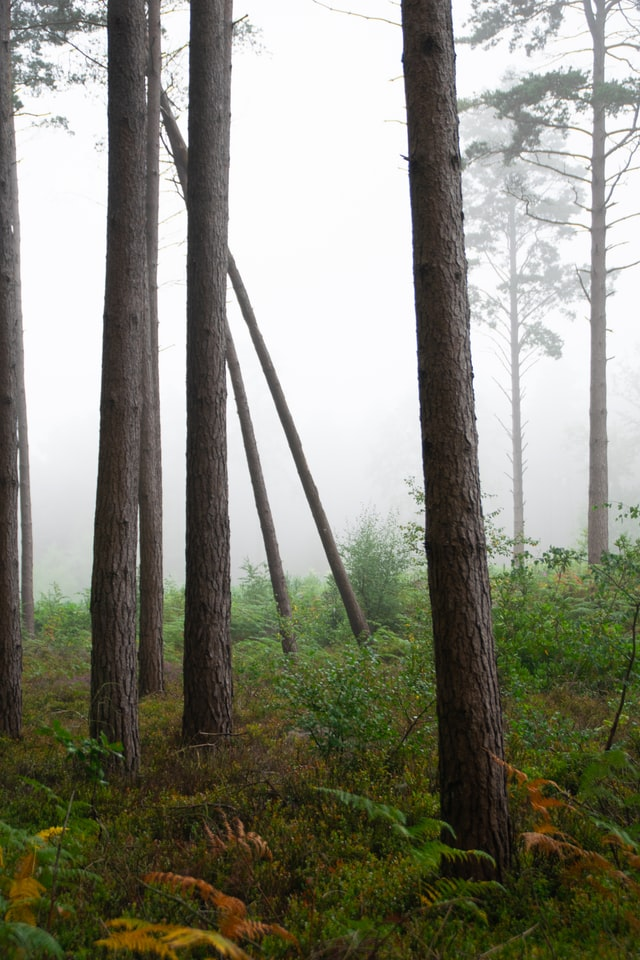
\includegraphics[trim=0cm 1cm 2.5cm 5cm, clip=true,width=0.85\textwidth]{images/harry-shelton-PmwG9GmNyaU-unsplash.jpg}
            
            \givecredit{Photo by \textlink{https://unsplash.com/@itsharryshelton}{Harry Shelton} on \textlink{https://unsplash.com}{Unsplash}}
        \end{column}
    \end{columns}
    
\end{frame}

%---------------------------------------------------------------
% 2. People
%---------------------------------------------------------------

\begin{frame}{Who's here?}
    
    \begin{columns}[t]
        \begin{column}{.3\textwidth}
    
            \begin{block}{Andy Clifton}
            \centering
            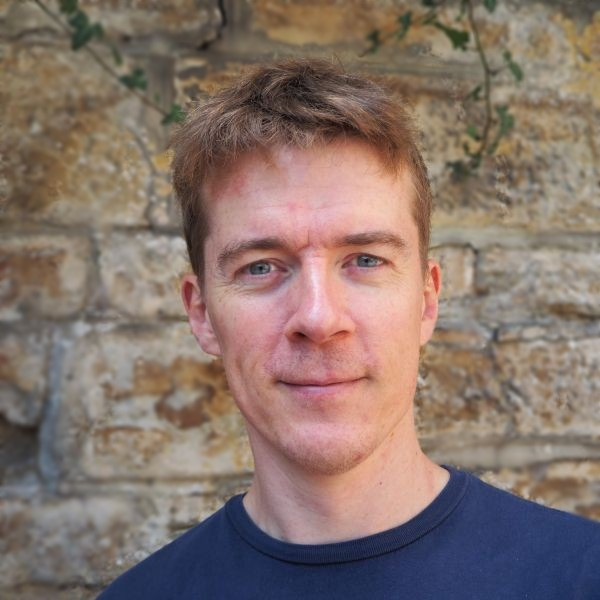
\includegraphics[width=0.8\textwidth]{images/Clifton_Headshot.jpg}\\
            IEA Wind Task 32\\ Operating Agent \\
            \orcid{0000-0001-9698-5083}
            \linkedin{http://www.linkedin.com/in/andyclifton}
            \end{block}
        \end{column}
   
        \begin{column}{.3\textwidth}
            \begin{block}{Nikola Vasiljevic}
            \centering
            
\includegraphics[width=0.8\textwidth]{images/Vasiljevic_Headshot.png}\\
            Special Consultant for Digitalization \\
            \orcid{0000-0002-9381-9693}
            \linkedin{https://dk.linkedin.com/in/niva83}
            \end{block}
        \end{column}
        
        \begin{column}{.3\textwidth}
            \begin{block}{And you}
            \centering
            {\fontsize{100}{120}\selectfont\faUsers}\\
            Please introduce yourselves!
            \end{block}
        \end{column}
    \end{columns}

\end{frame}
\section[The course]{The LIKE Open Science Course}
\stepcounter{subsection} %We don't use subsection titles, only frametitles
\label{sec:course}

%---------------------------------------------------------------
% 1. What is open science?
%---------------------------------------------------------------
\begin{frame}{What is this ``Open Science'' thing anyway?}

\begin{quotation}<1->
Open science is the movement to make scientific research and its dissemination accessible to all levels of an inquiring society, amateur or professional. \\
Open science is transparent and accessible knowledge that is shared and developed through collaborative networks.
\begin{flushright}
    \tiny{---\textlink{https://en.wikipedia.org/wiki/Open_science}{Wikipedia}}
  \end{flushright}
\end{quotation}

\begin{columns}
    \begin{column}{.45\textwidth}
    % it is...
        \begin{block}<2->{It is...}
            \begin{itemize}
                \item A philosophy
                \item A set of tools
                \item An old idea
            \end{itemize}
        \end{block}
    \end{column}
    
    \begin{column}{.45\textwidth}
    % it is not...
        \begin{block}<2->{It is not...}
            \begin{itemize}
                \item Difficult
                \item Expensive
                \item Rewarded directly
            \end{itemize}
        \end{block}
    \end{column}
    
\end{columns}

\end{frame}


%---------------------------------------------------------------
% 2. High-level goals
%---------------------------------------------------------------

% high-level goals
\begin{frame}{Course goals}

\begin{columns}[t]
    % LHS text
    \begin{column}{.45\textwidth}

    \textbf{We want you to be successful.}
    \vspace{3ex}
    

    This course will:
    \begin{itemize}
        \item Tell you about open science
        \item Give you a toolbox
        \item Help you use these tools
    \end{itemize}
    
    \end{column}

    % RHS image
    \begin{column}{.45\textwidth}

        \centering
        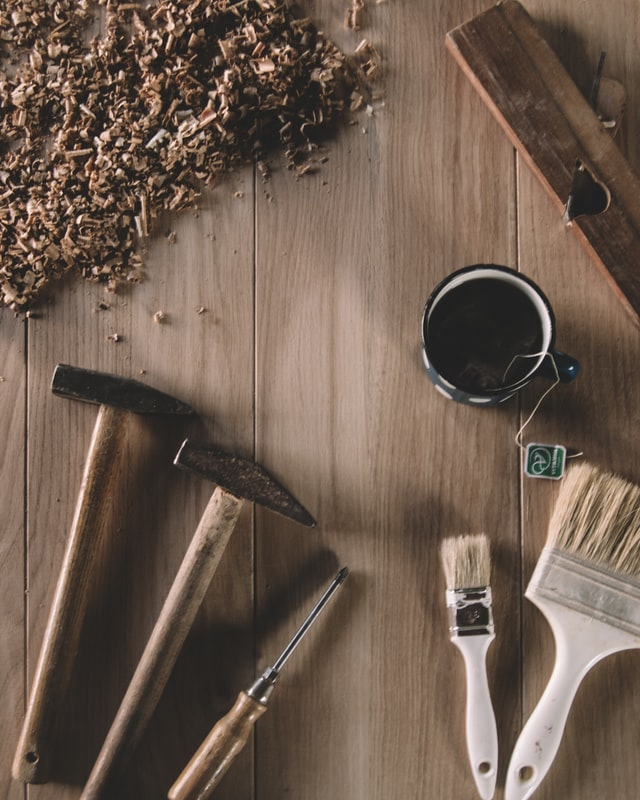
\includegraphics[width=0.8\textwidth]{images/milan-popovic-BmyXTxyDL-I-unsplash.jpg}
    
        \givecredit{\centering Photo by \textlink{https://unsplash.com/@itsmiki5?utm_source=unsplash&amp;utm_medium=referral&amp;utm_content=creditCopyText}{Milan Popovic} on \textlink{https://unsplash.com/s/photos/tools?utm_source=unsplash&amp;utm_medium=referral&amp;utm_content=creditCopyText}{Unsplash}}
    
    \end{column}

\end{columns}


\end{frame}

%---------------------------------------------------------------
% 3. Calendar
%---------------------------------------------------------------

\begin{frame}{Course outline}

\begingroup
\renewcommand{\arraystretch}{0.9} % Default value: 1
\setlength\tabcolsep{0pt}  % default value: 6pt
% Table based on https://github.com/LIKE-ITN/OpenScienceTrainingCourse/blob/master/readme.md#course-outline
\setlength{\fboxsep}{3pt}
\colorbox{uniSgray!10}{%

    \begin{tabular}{@{}p{0.35\textwidth}p{0.35\textwidth}p{0.3\textwidth}@{}}
        Seminar & Self-study & Deliverable \\
        \midrule
        1. \textlink{https://github.com/LIKE-ITN/OpenScienceTrainingCourse/blob/master/01_seminar1/readme.md}{Introducing open science} &  &  \\
         &  1. \textlink{https://github.com/LIKE-ITN/OpenScienceTrainingCourse/blob/master/selfstudy1.md}{Background reading} &  \\
        2. \textlink{https://github.com/LIKE-ITN/OpenScienceTrainingCourse/blob/master/seminar2.md}{Guiding principles} &  &  \\
         & 2. \textlink{https://github.com/LIKE-ITN/OpenScienceTrainingCourse/blob/master/selfstudy2.md}{Is your group's work FAIR?} &  \\
        3. \textlink{https://github.com/LIKE-ITN/OpenScienceTrainingCourse/blob/master/seminar3.md}{Open science and intellectual property} &  &  \\
         & 3. \textlink{https://github.com/LIKE-ITN/OpenScienceTrainingCourse/blob/master/selfstudy3.md}{Implementing open science} & \\
        4. \textlink{https://github.com/LIKE-ITN/OpenScienceTrainingCourse/blob/master/seminar3.md}{Communicating your science} &  &  \\
         & 4. \textlink{https://github.com/LIKE-ITN/OpenScienceTrainingCourse/blob/master/selfstudy4.md}{Communications strategies} &  \\
         &  & 1. \textlink{https://github.com/LIKE-ITN/OpenScienceTrainingCourse/blob/master/deliverable1.md}{Implementation case study} \\
         5. \textlink{https://github.com/LIKE-ITN/OpenScienceTrainingCourse/blob/master/seminar5.md}{What are data management plans and why do they matter?} &  &   \\
         & 5. \textlink{https://github.com/LIKE-ITN/OpenScienceTrainingCourse/blob/master/selfstudy5.md}{Draft a data management plan} &  \\
        Workshop: \textlink{https://github.com/LIKE-ITN/OpenScienceTrainingCourse/blob/master/workshop1.md}{Open science in LIKE} &  & \\
         & 6. \textlink{https://github.com/LIKE-ITN/OpenScienceTrainingCourse/blob/master/selfstudy6.md}{Revise data management plan} &  \\
         &  & 2. \textlink{https://github.com/LIKE-ITN/OpenScienceTrainingCourse/blob/master/deliverable2.md}{Data management plan} \\
         
    \end{tabular}
}\endgroup

\end{frame}

%---------------------------------------------------------------
% 3. Logistics - Office Hours, Questions, Etc.
%---------------------------------------------------------------

\begin{frame}{Course logistics}
    
    \begin{columns}
    \column{.45\textwidth}
   
        \begin{block}{Grading}
            \begin{itemize}
                \item No exams, but..
                \item Deliverables needed for a participation certificate.
            \end{itemize}
        \end{block}

        \begin{block}{Questions?}
            \begin{itemize}
                \item No office hours!
                \item Use slack and ask each other
            \end{itemize}
        \end{block}

    \column{.45\textwidth}
    
        \begin{block}{Errors, suggestions, corrections...}
            \begin{itemize}
                \item  \textlink{https://github.com/LIKE-ITN/OpenScienceTrainingCourse/issues}{Help improve the material}
            \end{itemize}
        \end{block}

        \begin{block}{Your feedback}
        This is a new course!
            \begin{itemize}
                \item Get in touch at any time
                \item Survey at the end
            \end{itemize}
        \end{block}

        \end{columns}
    
\end{frame}

\section[Who's data is it]{Let's talk about who owns (your) science}
\stepcounter{subsection} %We don't use subsection titles, only frametitles
\label{sec:ownership}

%---------------------------------------------------------------
% 1. What are the outputs?
%---------------------------------------------------------------

\begin{frame}{What are the outputs of science?}

% left empty for student input

\end{frame}

%---------------------------------------------------------------
% 2. Who's data is it?
%---------------------------------------------------------------
\begin{frame}{Who's data is it anyway?}

\begin{columns}[c]
    \begin{column}{0.45\textwidth}

    \begin{minipage}[t][.7\textheight]{\textwidth}

    Your intellectual output at work belong to your employer.
    \begin{itemize}
    \item It is their \emph{Intellectual Property} (IP).
    \end{itemize}
    
    \vfill
    
    IP can take many forms:
    \begin{itemize}
        \item Formalised through patents, trademarks, copyright,...
        \item Also found in papers, presentations, photos, videos, audio,...
    \end{itemize}
    
    \vfill
    
    \textbf{Using IP without permission is ``IP Infringement'' (not good).}
    \end{minipage}%
    
    \end{column}

    \begin{column}{0.45\textwidth}
        
\includegraphics[width=0.85\textwidth]{images/bermix-studio-F7DAQIDSk98-unsplash.jpg}
        \givecredit{Photo by \textlink{https://unsplash.com/@bermixstudio}{Bermix Studio} on \textlink{https://unsplash.com/s/photos/thief}{Unsplash}}
    \end{column}

\end{columns}

\end{frame}

%---------------------------------------------------------------
% 3. A quick detour - open source and open science
%---------------------------------------------------------------
\begin{frame}{A detour - open science and open source}

\begin{columns}[c]
    \begin{column}{0.35\textwidth}
        
        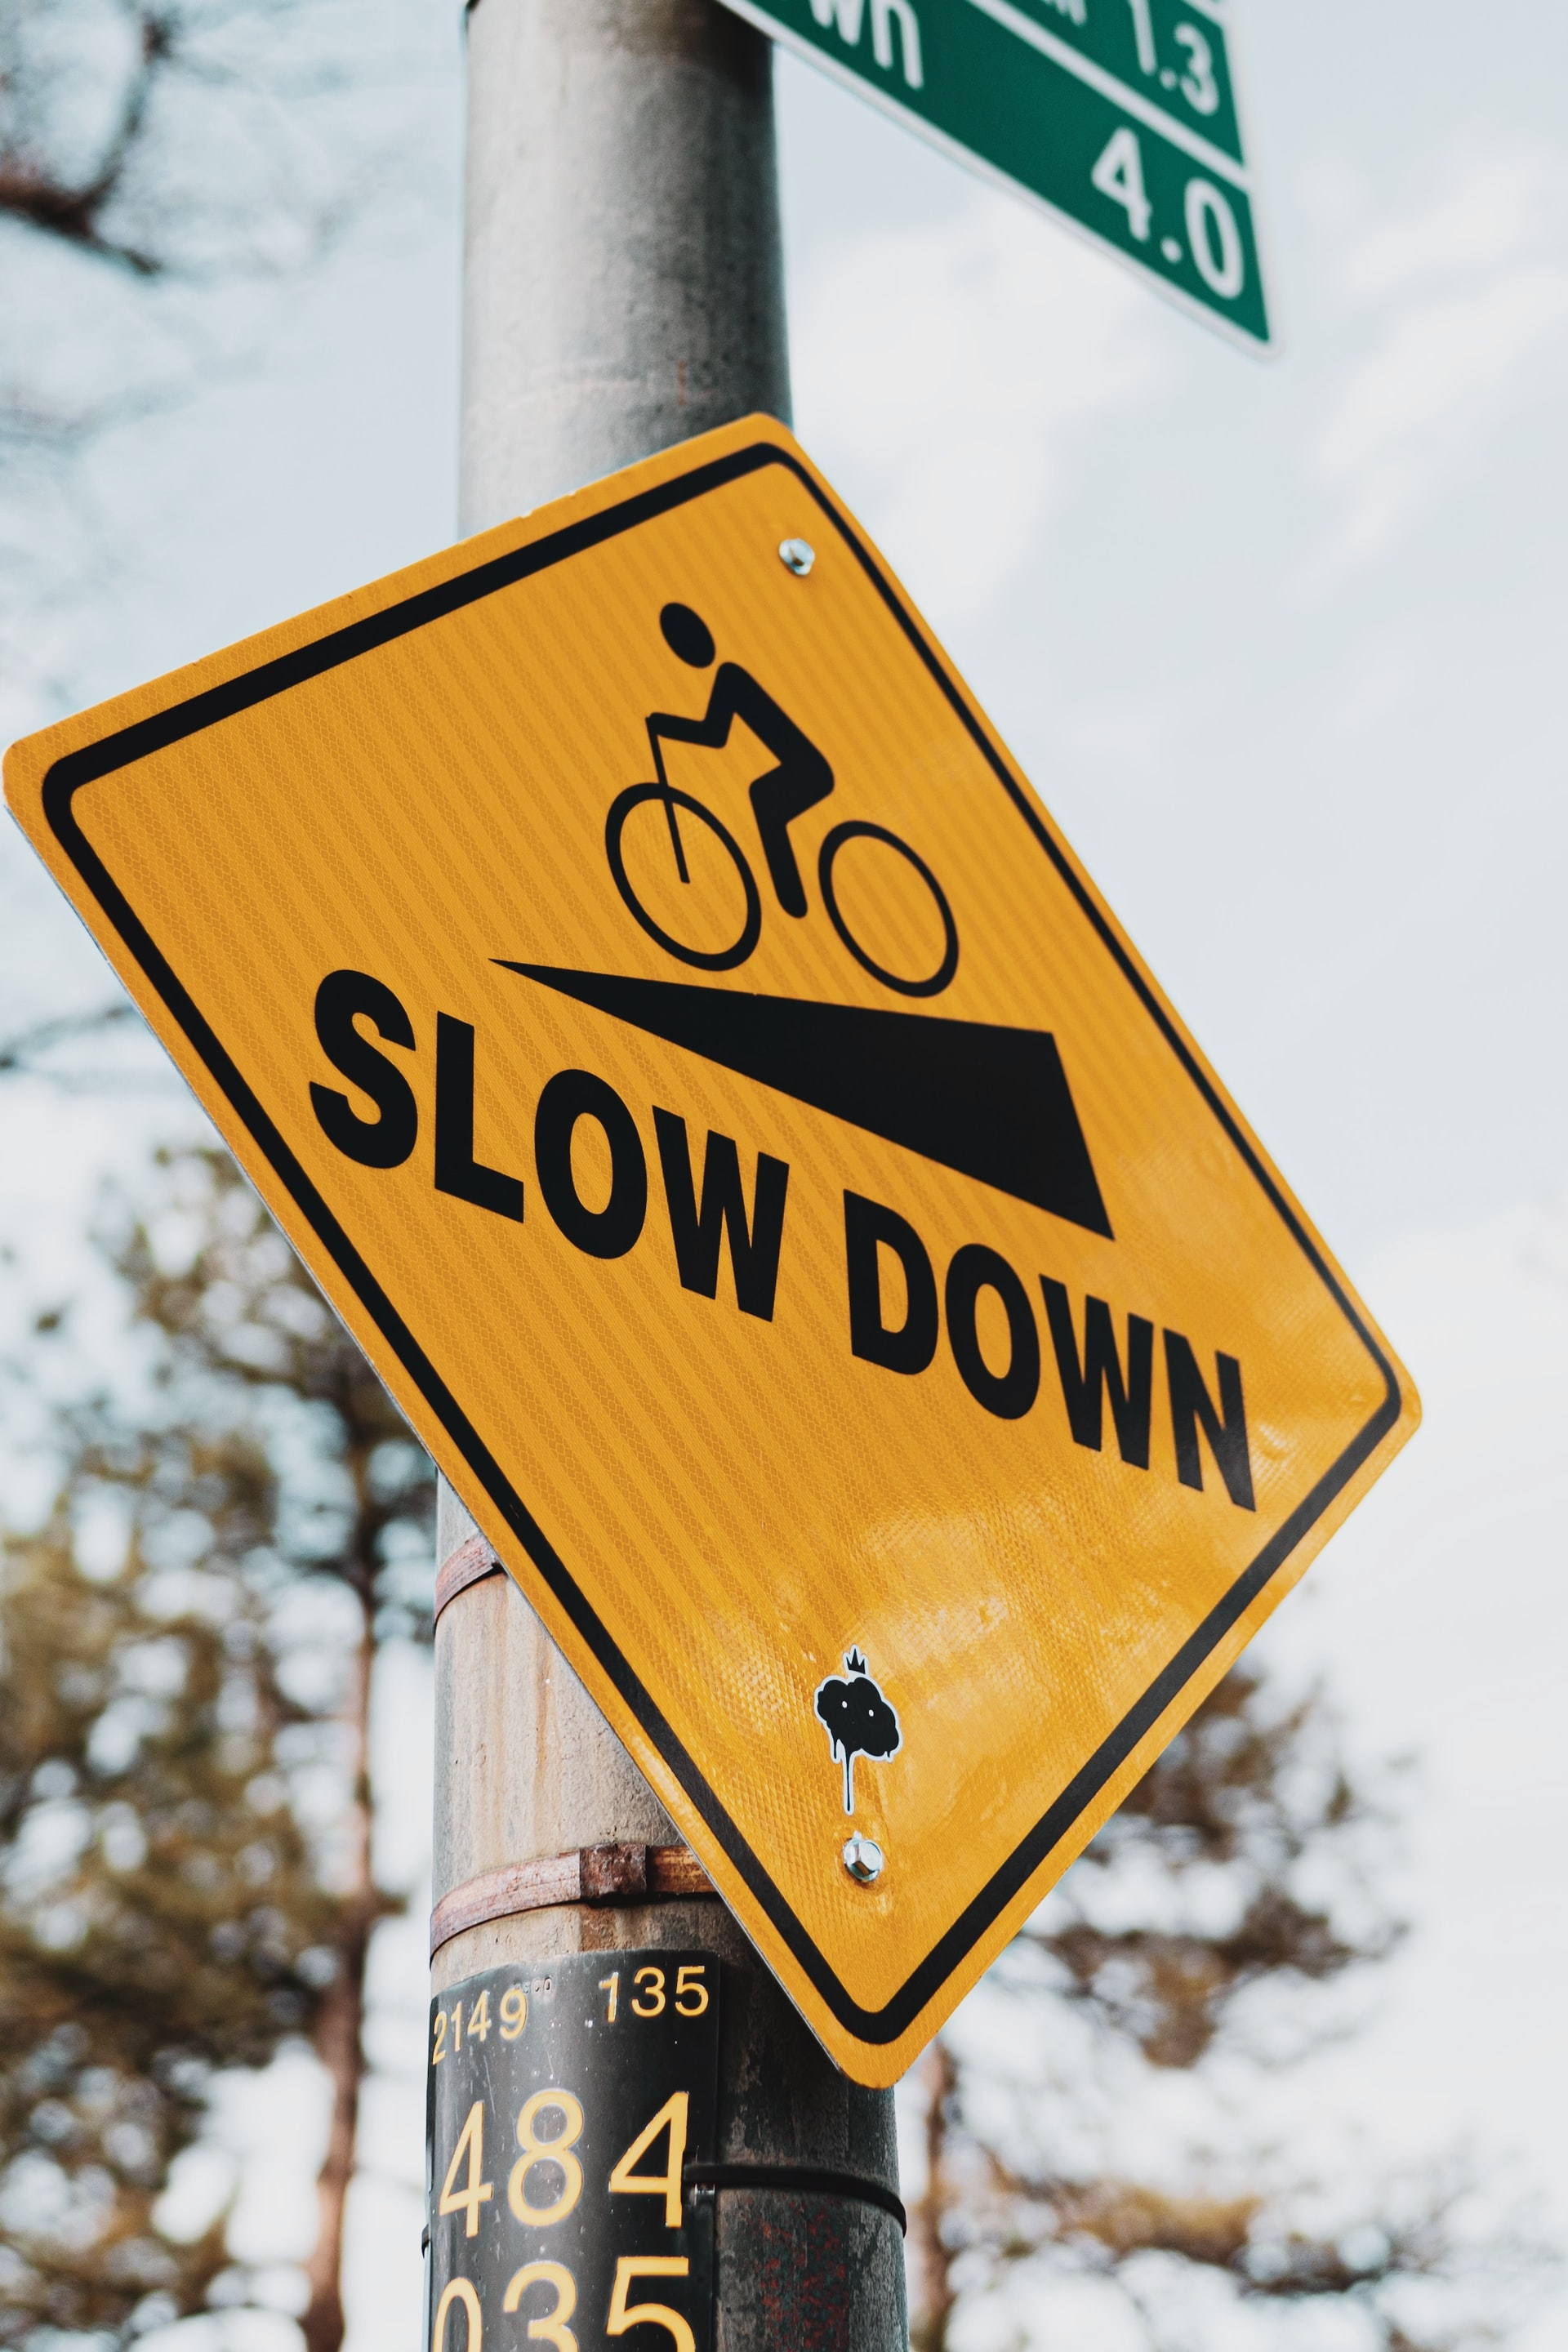
\includegraphics[width=0.85\textwidth]{images/logan-weaver-PJYOpJCcbRg-unsplash.jpg}
        
        \givecredit{Photo by \textlink{https://unsplash.com/@lgnwvr}{logan Weaver} on \textlink{https://unsplash.com/s/photos/warning}{Unsplash}}
        

    \end{column}
    
    \begin{column}{0.45\textwidth}

    Let's think about this:
    \begin{itemize}
        \item What's open source software?
        \item Is open source software free to use?
        \item Why would you have to pay for open-source software?
    \end{itemize}
    
    Making software open source helps open science, but isn't essential
    
    \end{column}
\end{columns}

\end{frame}


%---------------------------------------------------------------
% 4. How can I identify IP?
%---------------------------------------------------------------
\begin{frame}{Identifying IP}

\begin{columns}[c]

    \begin{column}{0.45\textwidth}
        {%
\setlength{\fboxsep}{0pt}%
\setlength{\fboxrule}{1pt}%
\fbox{%
        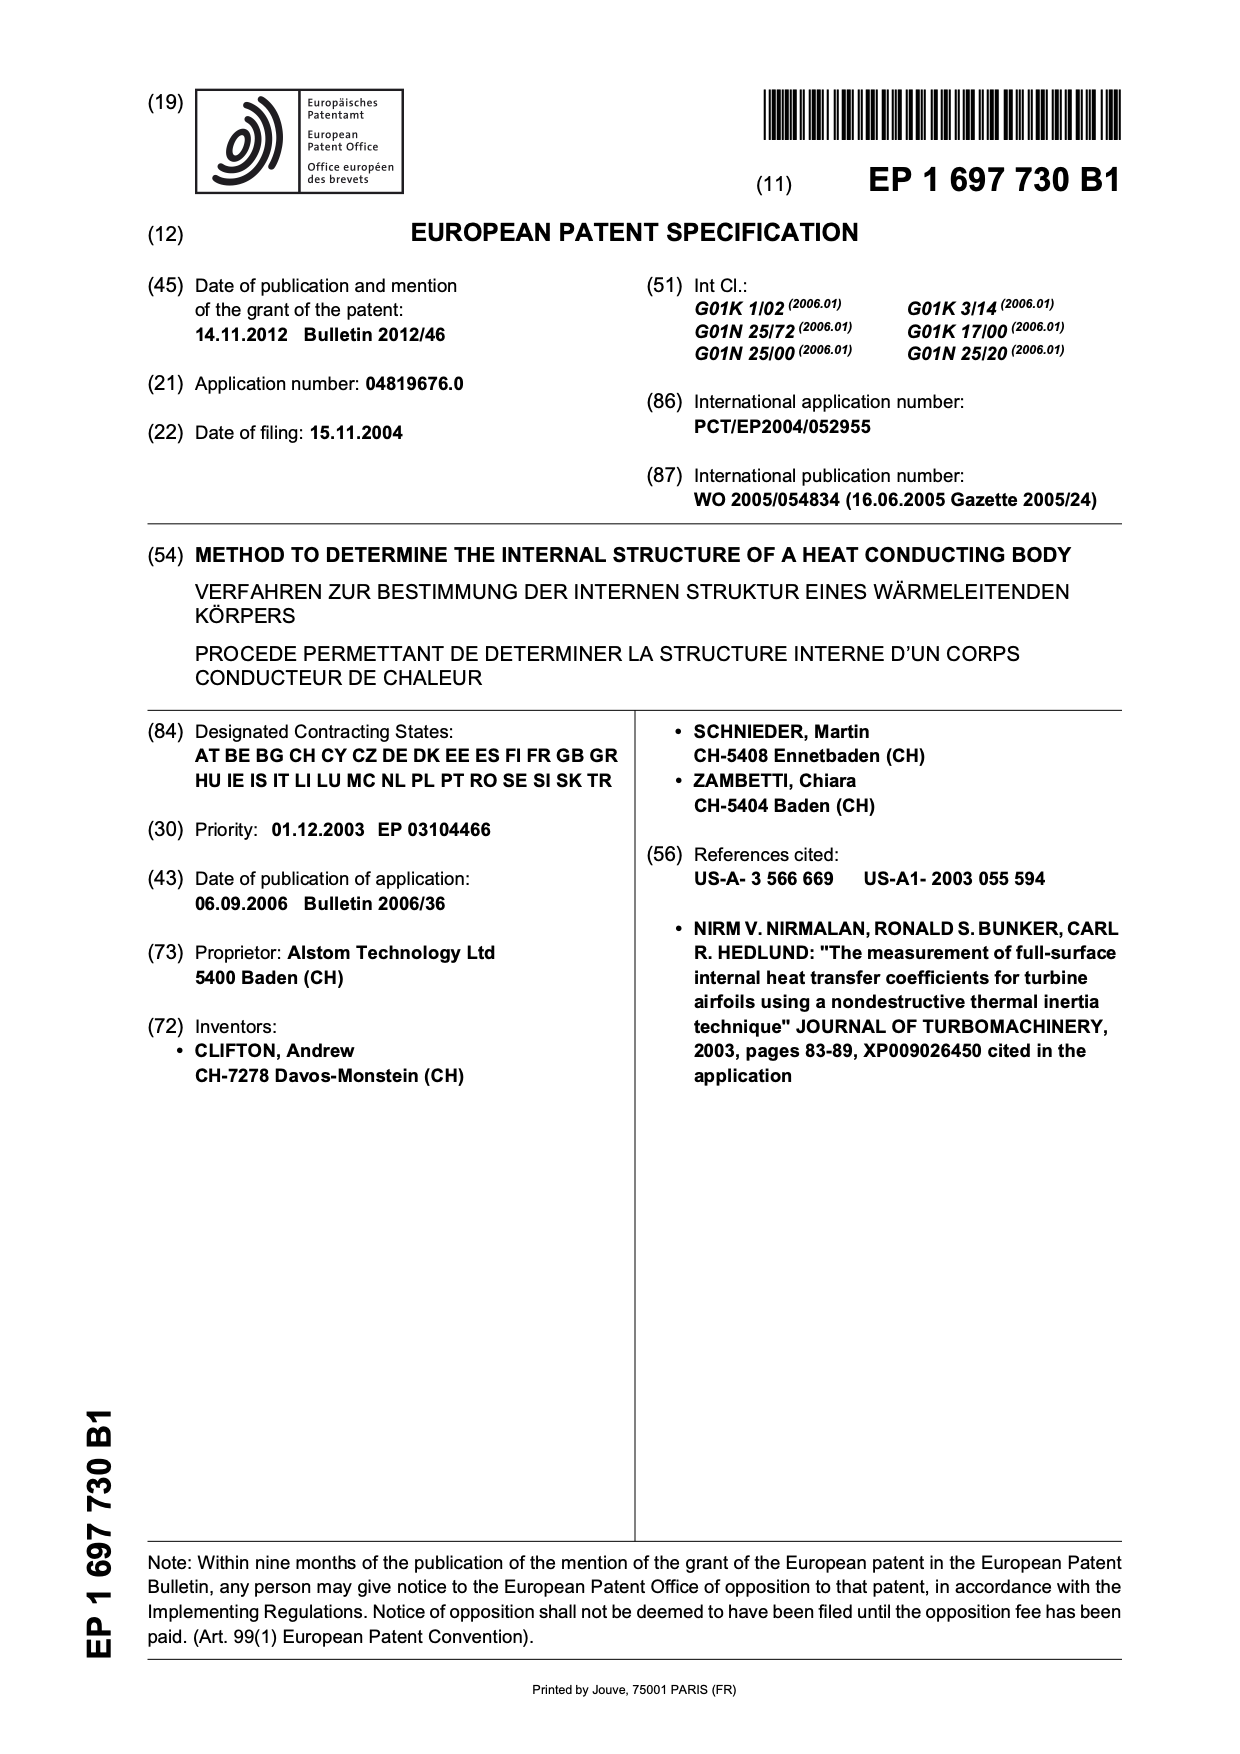
\includegraphics[width=0.75\textwidth]{images/EP1697730B1.png}
        }%
        }%
    \end{column}

    \begin{column}{0.45\textwidth}
    IP can protect solutions, form, and content:
    \begin{itemize}
        \item Patents
        \item Design rights or design patents
        \item Trademarks
        \item Copyright
    \end{itemize}
    
    But it is up to you to protect `trade secrets' from competitors!
    
    \end{column}

\end{columns}

\end{frame}

%---------------------------------------------------------------
% 5. How can I use it?
%---------------------------------------------------------------
\begin{frame}{Licenses tell people how they can use code or products}

Once you have protected your IP, you can think about sharing it

\vfill

\begin{columns}[c]

    \begin{column}{0.45\textwidth}
        \begin{block}{Created works?}
        
\includegraphics[trim=0 0 40 127, clip, width=\textwidth]{images/patrick-tomasso-Oaqk7qqNh_c-unsplash.jpg}\\
        Try \textlink{https://creativecommons.org/share-your-work/}{creative commons}.
        \end{block}
    \end{column}
    
    \begin{column}{0.45\textwidth}
        \begin{block}{Open-source software?}
        
\includegraphics[trim=0 0 40 127, clip, width=\textwidth]{images/chris-ried-ieic5Tq8YMk-unsplash.jpg}
        
        Try \textlink{https://choosealicense.com/}{ChooseALicense.com}
        \end{block}
    \end{column}
\end{columns}

\vfill

\centering{\textbf{Get a lawyer involved!}}

\vfill

\photocredit{Photos by \textlink{ href="https://unsplash.com/@impatrickt}{Patrick Tomasso} (left) and \textlink{https://unsplash.com/@cdr6934}{Chris Ried} (right) on \textlink{ href="https://unsplash.com/s/photos/book}{Unsplash}}

\end{frame}


%---------------------------------------------------------------
% 6. The COVID_19 pledge
%---------------------------------------------------------------
\begin{frame}{An example from the COVID-19 response}

\vfill

\begin{quotation}
Amazon, Facebook, Fujitsu, Hewlett Packard Enterprise, IBM, Intel, Microsoft, NASA JPL, Sandia National Laboratories, and Uber are among the dozens of companies and institutions that have used the Open COVID Pledge to make their patents and copyrights open to the public in support of solving the COVID-19 pandemic.
\begin{flushright}
    \tiny{---\textlink{https://creativecommons.org/2020/08/27/cc-ocp/}{Creative Commons Is Now Leading the Open COVID Pledge—Here’s What That Means. Creative Commons, 27 Aug 2020}}
  \end{flushright}
\end{quotation}

\vfill

But can you make money like this?

\end{frame}

%---------------------------------------------------------------
% 7. Making money from openness
%---------------------------------------------------------------
\begin{frame}{How can you make money from open science?}

\begin{columns}[c]

    \begin{column}{0.45\textwidth}
        
\includegraphics[width=\textwidth]{images/IBM_linux.png}\pause
    \end{column}
    
    \begin{column}{0.45\textwidth}
        Like any business, you need to add value.
        \begin{itemize}
            \item Deploy it for customers
            \item Provide training
            \item Customize it
            \item Develop add-ons
            \item Create an ecosystem
        \end{itemize}
    \end{column}
    
\end{columns}

\end{frame}

%---------------------------------------------------------------
% 8. Making money from openness (II)
%---------------------------------------------------------------
\begin{frame}{How can you make money from open science?}

\begin{columns}[c]

    \begin{column}{0.45\textwidth}
        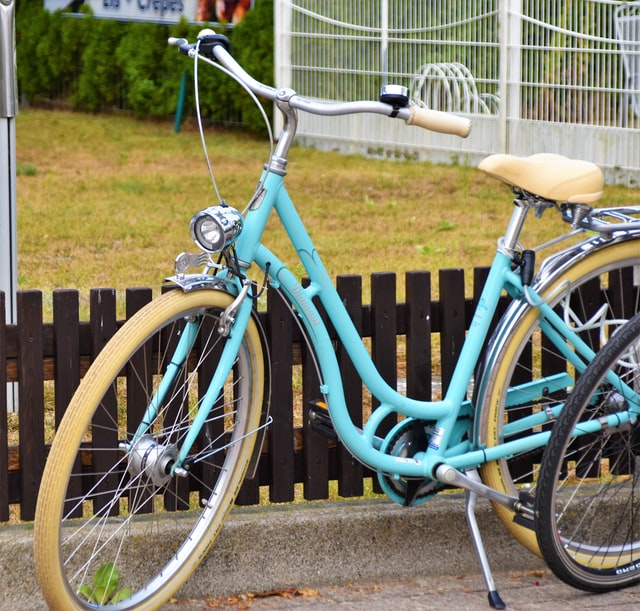
\includegraphics[width=\textwidth]{images/waldemar-brandt-FiK8jopQh8-unsplash.jpg}
        \givecredit{Photo by \textlink{https://unsplash.com/@waldemarbrandt67w}{Waldemar Brandt} on {https://unsplash.com/s/photos/bike}{Unsplash}}\pause
    \end{column}
    
    \begin{column}{0.45\textwidth}
        Good solutions are
        \begin{itemize}
            \item Flexible but focused
            \item Modular
            \item Easy to use
        \end{itemize}
    \end{column}
    
\end{columns}

\end{frame}

\section[Closing]{Closing thoughts}
\label{sec:closing}

%---------------------------------------------------------------
% 1. Summary
%---------------------------------------------------------------
\begin{frame}{Seminar summary}

	\begin{columns}[c]
		% lessons
		\begin{column}{.45\textwidth}
		    You've learned:
		    \begin{itemize}
			    \item About the course
			    \item A first definition for ``open science''
			    \item How openness helps fight COVID-19
			    \item Some challenges with being open
		    \end{itemize}
		\end{column}

		\begin{column}{.45\textwidth}
		
		    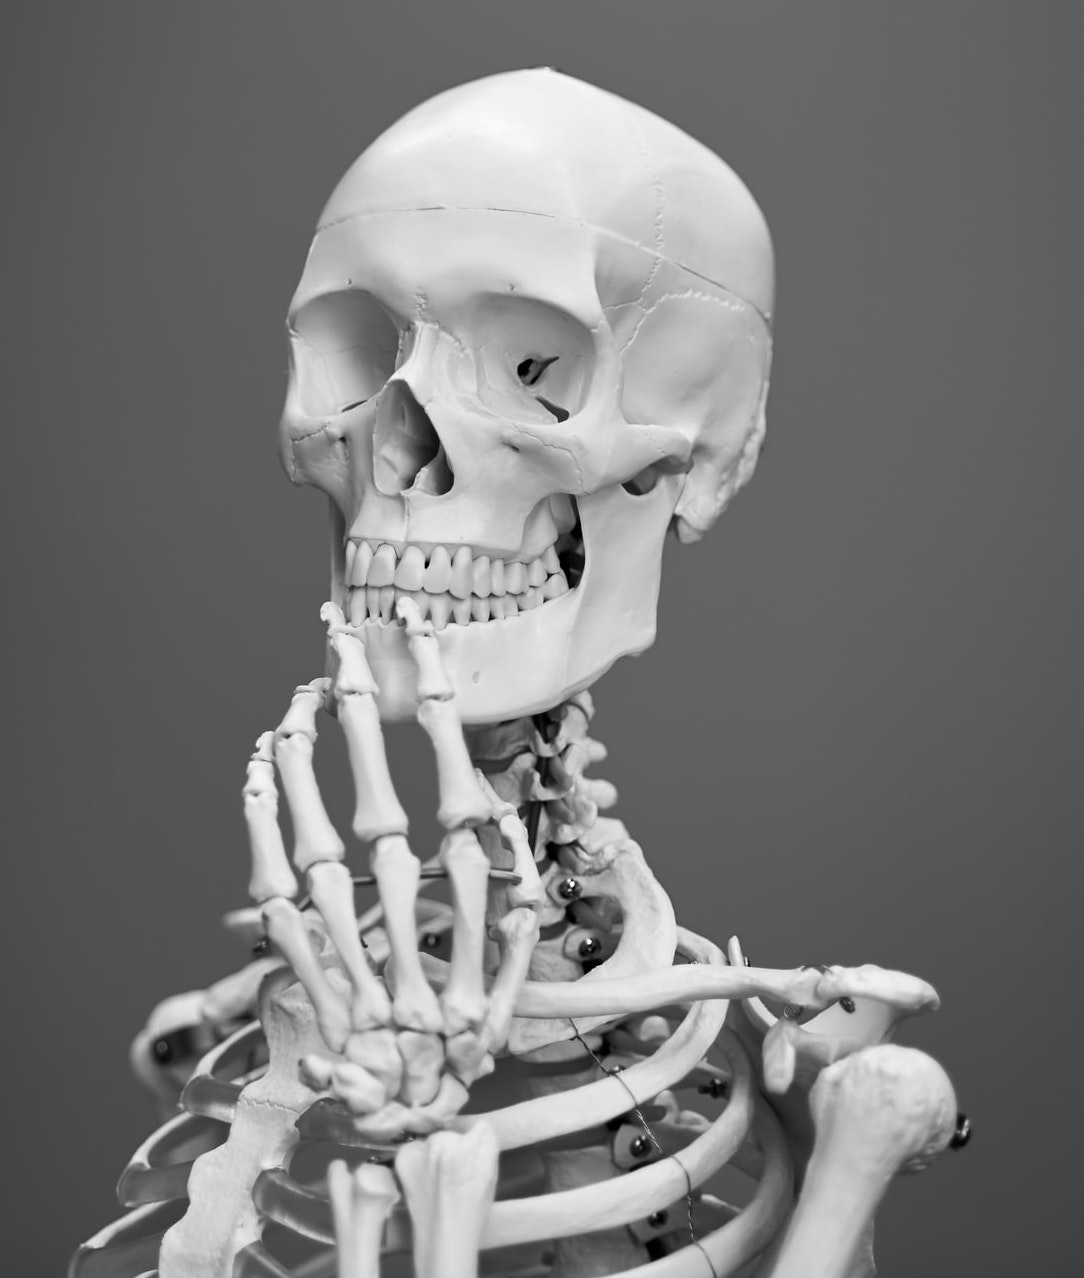
\includegraphics[width=0.85\textwidth]{images/mathew-schwartz-8rj4sz9YLCI-unsplash-crop.jpg}
		    
		    \givecredit{%
		        \centering
		        Photo by \textlink{https://unsplash.com/@cadop}{Mathew Schwartz} on \textlink{https://unsplash.com/s/photos/thinking}{Unsplash}}
		\end{column}
		
	\end{columns}

\end{frame}

%---------------------------------------------------------------
% 2. Next steps
%---------------------------------------------------------------

\begin{frame}{What to do now}

	\begin{columns}[t]
		\column{.45\textwidth}
		\begin{block}{Self study 1: Background reading}
			Read about how open science has been used to fight COVID-19, for example...
			\begin{itemize}
				\item \textlink{https://www.nature.com/articles/d41586-020-01246-3}{Open science takes on the coronavirus pandemic (Nature, 2020)}
				\item \textlink{https://www.rd-alliance.org/data-sharing-time-pandemic-patterns-preview-rda-covid-19-group-results}{``Data Sharing in a Time of Pandemic''} (Patterns, 2020)
				\item \textlink{https://home.cern/news/news/computing/open-science-against-covid-19-how-zenodo-and-openaire-support-scientists}{``Open Science against COVID-19: how Zenodo and OpenAIRE support the scientists''} (CERN, 2020)
			\end{itemize}
		\end{block}

		\column{.45\textwidth}
		\begin{block}{Seminar 2: Guiding principles}
			What are the basic principles of open science? How can you implement them, and what do they mean for your organisation?
			\begin{itemize}
				\item \textlink{https://github.com/LIKE-ITN/OpenScienceTrainingCourse/blob/master/seminar2.md}{Seminar materials on GitHub}
			\end{itemize}
		\end{block}

	\end{columns}

\end{frame}

%---------------------------------------------------------------
% 3. Let's make this open
%---------------------------------------------------------------
\begin{frame}{Let's make this presentation open}

	\begin{columns}[t]
		\begin{column}{.45\textwidth}
		    \centering
		    
\includegraphics[height=1.5cm]{images/1280px-FAIR_data_principles.jpg}

		    \givecredit{\centering Image source: \textlink{https://en.wikipedia.org/wiki/FAIR_data#/media/File:FAIR_data_principles.jpg}{Wikimedia}. Credit: \textlink{https://commons.wikimedia.org/w/index.php?title=User:SangyaPundi}{SangyaPundir}. \\
		    Reused under the \textlink{https://creativecommons.org/licenses/by-sa/4.0}{CC BY-SA 4.0 license}}
		\end{column}

		\begin{column}{.45\textwidth}
		    \centering
		    
\includegraphics[height=1.5cm]{images/cc-by-sa.png}
        \end{column}
	\end{columns}

	\begin{columns}[t]
		\begin{column}{.45\textwidth}
		    \centering
		% Findable
		    \begin{block}{Findable}
			    This presentation has a DOI:
		    \end{block}

		    % accessible
		    \begin{block}{Accessible}
			    This presentation is archived at Zenodo.org. \\
			    The source code is available through GitHub.
		    \end{block}
        \end{column}

		\begin{column}{.45\textwidth}
		    \centering
		    \begin{block}{Interoperable}
			    This material is produced using the \LaTeX\space `Beamer' package.
		    \end{block}

		    \begin{block}{Reusable}
			    This material is reusable under the \textlink{https://creativecommons.org/licenses/by/4.0/}{CC-BY-4.0 license}.
		    \end{block}
        \end{column}
	\end{columns}
\end{frame}

% corporate identity
\finalslide{clifton@ifb.uni-stuttgart.de}{+49 711 685 683 25}{www.uni-stuttgart.de/windenergie}

\end{document}




%%% Local Variables:
%%% mode: latex
%%% TeX-master: t
%%% End:
